\documentclass[]{article}

\usepackage{tikz}
\usepackage{amsmath}
\usepackage{amsfonts}
\usepackage{amssymb}
\usepackage{tkz-base}
\usepackage{tkz-euclide}
\usepackage{xcolor}
\usepackage{pgfplots}
\usepackage{graphicx}

% Required package
\usetikzlibrary{positioning}
\usetikzlibrary{svg.path}
\usetikzlibrary{arrows}
\usetikzlibrary{shapes.geometric,calc}

\newdimen\XCoord
\newdimen\YCoord
\newcommand*{\ExtractCoordinate}[1]{\path (#1); \pgfgetlastxy{\XCoord}{\YCoord};}%

%opening
\title{Indirect Compliance Control\linebreak a.k.a. Position--based Compliance Control\linebreak a.k.a. Admittance Control}
\author{Glen Henshaw\\Craig Carignan}

\begin{document}

\maketitle

\section{Intro}
So far we've discussed how to control the position of a robot, either in operational space or configuration space. This works fine when the robot is moving around in free space. But when it needs to physically interact with the environment -- say by inserting a part into a hole, or turning a screw, or picking up a Mars rock -- then we may suddenly be pretty concerned about the forces the robot exerts (or doesn't exert) as well as what its position is.

There are a variety of schemes for controlling force with a robot, but two are currently winning: ``indirect compliance control'', aka admittance control, and ``direct compliance control'', aka impedance control. Today we're going to discuss indirect compliance control.

\section{Compliance Control}
The basic idea behind compliance control is that you want to make the robot emulate the dynamic behavior of a forced spring--mass--damper system. We've discussed SMD systems \textit{ad nauseum} in this class, but this is a little different. Here, instead of trying to view the dynamics of our system as a SMD in order to control the position, here we want to make use of another view of SMD systems, which is that they \textbf{trade off position and force}.
\pagebreak

Here's a spring--mass--damper system:
\begin{figure}[h!]
\centering
 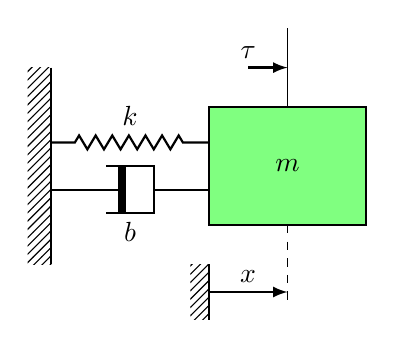
\begin{tikzpicture}[every node/.style={outer sep=0pt},thick,
 mass/.style={draw,thick},
 spring/.style={thick,decorate,decoration={zigzag,pre length=0.3cm,post
 length=0.3cm,segment length=6}},
 ground/.style={fill,pattern=north east lines,draw=none,minimum
 width=0.75cm,minimum height=0.3cm},
 dampic/.pic={\fill[white] (-0.1,-0.3) rectangle (0.3,0.3);
 \draw (-0.3,0.3) -| (0.3,-0.3) -- (-0.3,-0.3);
 \draw[line width=1mm] (-0.1,-0.3) -- (-0.1,0.3);}]

  \node[mass,minimum width=2cm,minimum height=1.5cm,fill=green!50] (m1) {$m$};
   \node[left=2cm of m1,ground,minimum width=3mm,minimum height=2.5cm] (g1){};
  \draw (g1.north east) -- (g1.south east);

  \draw[spring] ([yshift=3mm]g1.east) coordinate(aux)
   -- (m1.west|-aux) node[midway,above=1mm]{$k$};

  \draw ([yshift=-3mm]g1.east) coordinate(aux')
   -- (m1.west|-aux') pic[midway]{dampic} node[midway,below=3mm]{$b$};
 
  \foreach \X in {1}  
  {\draw[thin] (m\X.north) -- ++ (0,1) coordinate[midway](aux\X);
   \draw[latex-] (aux\X) -- ++ (-0.5,0) node[above]{$\tau$}; 
   \draw[thin,dashed] (m\X.south) -- ++ (0,-1) coordinate[pos=0.85](aux'\X);
   \draw[latex-] (aux'\X) -- ++ (-1,0) node[midway,above]{$x$}
    node[left,ground,minimum height=7mm,minimum width=1mm] (g'\X){};
   \draw[thick] (g'\X.north east) -- (g'\X.south east);
  }

\end{tikzpicture}
\end{figure}

Imagine what would happen if you had chosen your spring and damping gains, and then perturbed the system by exerting a force $\tau_{1}$ on it. It would move, of course, but it would do so in a way that was dependent on $k_{1}$, $b_{1}$, and $m_{1}$. This is referred to as ``mechanical impedance'', and is a measure of how much a system resists motion when a force is applied.

One very effective way of thinking about robotic contact operations is to consider how much mechanical admittance or impedance they require. With the right controller structure, we can build this in by choosing the right gains. Of course, in order to make this work we need to sense force as well as position, so we'll generally need either a force--torque sensor mounted somewhere in the system, or we'll need torque sensors mounted in the joints. Indirect compliance control is almost always implemented using a 6--axis force--torque sensor mounted in the wrist or end effector, for reasons we'll get into a bit later.

\subsection{Example: the Salisbury Stiffness Controller}

Suppose we just want to control the stiffness of the arm as it interacts with the environment. We want to do this around all six axes, x--y--z and roll--pitch--yaw. In other words, we want to enforce the following:
\begin{displaymath}
 \underline{F} = K_{p_{x}} \underbrace{(x_{d} - x)}_{\delta x}
\end{displaymath}
This is called ``stiffness control'' instead of ``impedance control'' because we are only specifying $K_{p}$. What controller achieves this Cartesian stiffness?

\begin{eqnarray}
 \dot{x} & = & J\dot{\theta} \cong J\ \delta\underline{\theta}\ \  \leftarrow\ \  \text{Good for small $\delta x$} \nonumber \\
 \underline{F} & = & K_{p_{x}}\ \delta\underline{x}\ \  \Rightarrow\ \  \underline{F} = K_{p_{x}}J\ \delta\underline{\theta} \nonumber \\
 \underline{\tau} & = & J^{T}\underline{F}\ \ \Rightarrow\ \ \underline{\tau} = \underbrace{J^{T}(\underline{\theta})K_{p_{x}}J(\underline{\theta})}_{K_{p\theta} (\underline{\theta})}\ \delta\underline{\theta} \nonumber
\end{eqnarray}

So a potential control law is:
\begin{displaymath}
 \underline{\tau} = \underbrace{J^{T}(\underline{\theta})K_{p_{x}}J(\underline{\theta})}_{K_{p\theta} (\underline{\theta})}\underline{\tilde{\theta}} + K_{v}\dot{\tilde{\underline{\theta}}}
\end{displaymath}
where the final term just adds some constant (in Cartesian space) damping to make the system stable. Note that $K_{v}$ is a constant.

It's important to note that $K_{p\theta}$ is in general much much lower than the $K_{p}$ gain for a position control PD control law. This means that the Salisbury stiffness controller is much worse at rejecting disturbances than a position controller would be. We have sacrificed positional accuracy for compliance. In some sense this is unavoidable.

Of course, you could try to add a model term to a controller like this to try to at least cancel out ``disturbances'' that are a result of the manipulator dynamics and environmental forces you can model, like gravity. There's a considerable amount of research in this area.

\section{Indirect Compliance Control}

Here is a block diagram of a robotic system that's set up for indirect compliance control:

\begin{figure}[h!]
 \centering
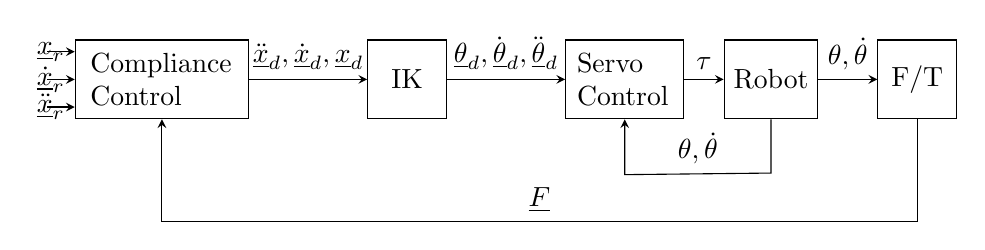
\begin{tikzpicture}
 % Sum shape
 \node[draw,
        minimum width=2.2cm,
        minimum height=1cm,
        ] (CC) at(0,0){\parbox[t]{0.15\linewidth}{Compliance\\Control}};
        
 \node[draw, 
        minimum width=1cm,
        minimum height=1cm,
        right=1.5cm of CC
        ] (IK) {IK};

% Controller
\node [draw,
    minimum width=1.5cm,
    minimum height=1cm,
    right=1.5cm of IK
]  (controller) {\parbox[t]{0.1\linewidth}{Servo\\Control}};
 
% System H(s)
\node [draw,
    minimum width=1cm, 
    minimum height=1cm,
    right=0.5cm of controller
] (system) {Robot};

\node[draw, minimum width=1cm,
            minimum height=1cm,
            right=0.75cm of system] (ft) {F/T};
  
% Arrows with text label
%\draw[-stealth] (trajgen.north east) -- (controller.north west)
%    node[midway,above]{$\Omega$};
\draw[-stealth] (CC.east) -- (IK.west) node[midway, above]{$\underline{\ddot{x}}_{d}, \underline{\dot{x}}_{d}, \underline{x}_{d}$};
\draw[-stealth] (IK.east) -- (controller.west)
    node[midway,above]{$\underline{\theta}_{d}, \dot{\underline{\theta}}_{d}, \ddot{\underline{\theta}}_{d}$};
 
\draw[-stealth] (controller.east) -- (system.west) 
    node[midway,above]{$\tau$};

\draw[-stealth] (system.east) -- (ft.west) 
    node[midway,above]{$\theta, \dot{\theta}$};

\ExtractCoordinate{controller.south}
\draw[-stealth] (system.south) -- ++ (0,\YCoord-5) -- (\XCoord, \YCoord-20) node[midway,above]{$\theta, \dot{\theta}$} -- (controller.south);

\ExtractCoordinate{ft.south}
\draw[-stealth] (ft.south) -- (\XCoord, \YCoord-37) -- node[midway,above]{$\underline{F}$}  (0, \YCoord-37) -- (CC.south);

\ExtractCoordinate{CC.west}
\draw[-stealth] (\XCoord-10, \YCoord) -- (\XCoord, \YCoord) node[left] {$\underline{\dot{x}}_{r}$};
\draw[-stealth] (\XCoord-10, \YCoord+10) -- (\XCoord, \YCoord+10) node[left] {$\underline{x}_{r}$};
\draw[-stealth] (\XCoord-10, \YCoord-10) -- (\XCoord, \YCoord-10) node[left] {$\underline{\ddot{x}}_{r}$};

\end{tikzpicture}
\end{figure}

What we've done here, unlike the stiffness controller above, is add an outer control loop to our existing architecture, which consists of a compliance control block and an inverse kinematics module, and an inner servo loop that controls position. Note that the inner loop can in theory be any of the control schemes we've talked about previously -- linear control, gain scheduling, or computed torque, among others.

The outer compliance control law looks like a spring--mass--damper system driven by a changing setpoint that we've labeled $\underline{x}_{r}$, which stands for ``reference trajectory'':
\begin{eqnarray}
 \underline{F} & = & K_{m}\left(\ddot{\underline{x}}_{r} - \ddot{\underline{x}}_{d}\right) + K_{v}\left(\underline{\dot{x}}_{r} - \underline{\dot{x}}_{d}\right) + K_{p}\left(\underline{x}_{r} - \underline{x}_{d}\right)  \nonumber \\
 \Rightarrow \ddot{\underline{x}}_{r} & = & K_{m}^{-1}\left[\underline{F} - K_{v}\left(\underline{\dot{x}}_{r} - \underline{\dot{x}}_{d}\right) - K_{p}\left(\underline{x}_{r}-\underline{x}_{d}\right) + K_{m}\underline{\ddot{x}}_{d}\right] \label{CC1}
 \end{eqnarray}
where $K_{m}$, $K_{v}$, and $K_{p}$ are virtual mass, damping, and stiffness gains that we want our system to emulate. In Equation \ref{CC1}, $\underline{F}$ is the \textit{sensed} force/torque vector coming from our force--torque sensor, and the output of the compliance control block is $\underline{\ddot{x}}_{d}$, $\underline{\dot{x}}_{d}$, and $\underline{x}_{d}$, the trajectory sent to the IK and then the servo control blocks. So we are integrating a differential equation in the outer loop that is in a sense simulating the behavior of a SMD system driven by the sensed force, and we are sending the trajectory that that simulated SMD would take to our servo loop to get the robot to follow the trajectory of the simulated system.

The main advantage of this type of compliance control is that it builds on all of the machinery we already have -- inverse kinematics and position--based servo control. Virtually all industrial robots already have all of this, so you can in general retrofit any existing robot arm to implement this type of compliance control, which accounts for its historical popularity.

There are a number of practical challenges with indirect compliance control. One is that, almost by definition, the stiffness gain $K_{p}$ is set pretty low -- you want your system to be compliant, after all. This means that disturbances that enter Equation \ref{CC1} -- say from bias or noise in the F/T sensor -- will significantly perturb the tracking of the reference trajectory. In point of fact, gravity compensation is very important here, because the F/T sensor \textit{will} sense gravity and respond to it. So you generally need to calculate and subtract off gravitational forces, and that can be challenging because it implies precise knowledge of the mass and inertia properties of anything distal from the F/T sensor, such as (for instance) the end effector and anything it may be holding.

A more subtle problem is that we are implicitly assuming that the inner control loop is capable of perfectly tracking $\underline{x}_{d}$. If it doesn't then the sensed forces won't track what the simulated SMD system in the compliance control block is ``expecting''. This will at the very least degrade the performance of the system, and can cause the system to become unstable. In fact, this problem gets worse as the desired compliance increases, e.g. as we tune $K_{p}$ and $K_{d}$ to simulate a softer SMD system. Intuitively this is because softer systems react more quickly to sensed forces, and so we are asking the arm to move faster and faster as the magnitudes of $K_{p}$ and $K_{d}$ become smaller. At some point we'll simply exceed the bandwidth of the arm and servo control enough that the sensed forces $\underline{F}$ will as a result exceed 90 degrees out of phase with the commanded trajectory $\underline{x}_{d}$; at this point the system becomes unstable and tends to try to beat itself to death against whatever contact point is available. This phenomenon occurs frequently enough that it has a name, ``contact instability''.

Stability of indirect compliance control is also negatively affected by the loop rate and whatever computational lag is present. The required loop rate is dependent on how compliant the robot is expected to be and on the natural mechanical compliance of the contact (including the mechanical compliance of the arm, the mechanical compliance of the tool, and the environment).

General guidelines for a working indirect compliance control system include:\begin{enumerate}
    \item Loop rates of 40--1000 Hz
    \item Loop latency of $< 20$ ms,(ideally $< 10$ ms)
    \item Significantly overdamped, e.g. $\|K_{v}\| > \|K_{p}\|$
\end{enumerate}

The required loop rate sometimes confuses people. In general, a serial link manipulator with a well--tuned servo controller has a bandwidth of around 1-5 Hz. Why, then would we ever need an outer loop rate of greater than 50 Hz, which implies a decade of separation? After all, the robot can't track trajectories that have frequency components of greater than 5 Hz.

The explanation of this phenomenon is that the bandwidth of a system is a function of \textit{what output is being measured}. When we say that a robot arm has a bandwidth of (say) 2 Hz, we are usually referring to its ability to track a position trajectory. In other words we are measuring position.

Recall, though, that Hooke's Law relates position to force:
\begin{displaymath}
    \underline{F} = -K_{e}\underline{x}
\end{displaymath}
where here, $K_{e}$ is the \textit{environmental} stiffness, e.g. it's the stiffness of whatever the robot is pushing against. If this is, for instance, a modest cantilevered steel beam has an equivalent spring stiffness of ~20,000 N/m, and a three--foot concrete pillar supported at both ends can have an equivalent spring stiffness of 9,000,000 N/m (if Google is to be believed!) or more. Therefore, very small motions of the end effector when in contact with a stiff environment result in absolutely enormous forces. If we measure the bandwidth of the robot as a force producing device, the Bode plot we would get when we measured position would be multiplied by the equivalent spring stiffness of the environment, which ``moves'' the Bode plot of the system up by this amount. As a consequence, there is a large increase in bandwidth. 

In practice, the actual bandwidth of the arm as a force producing device cannot be this high because it is limited by the most compliant mechanism in the robot--environment chain, and this is almost always the compliance of the robot's actuator, which is considerably less stiff than a cantilevered steel beam -- but it's still high unless the arm is specifically engineered with mechanical compliance in it.

\end{document}
